\section{Validation}
\label{sec:Validation}
	\subsection{Time-dependent energy consumption}
	The measurements of the energy consumptions has been done on a 64-bits computer, with 6GB of RAM and running Intel(R) Core(TM) i5-4210H CPU @ 2.90GHz processor. Results generated by PowerAPI are entered in the following graph :
\begin{figure}[H]
	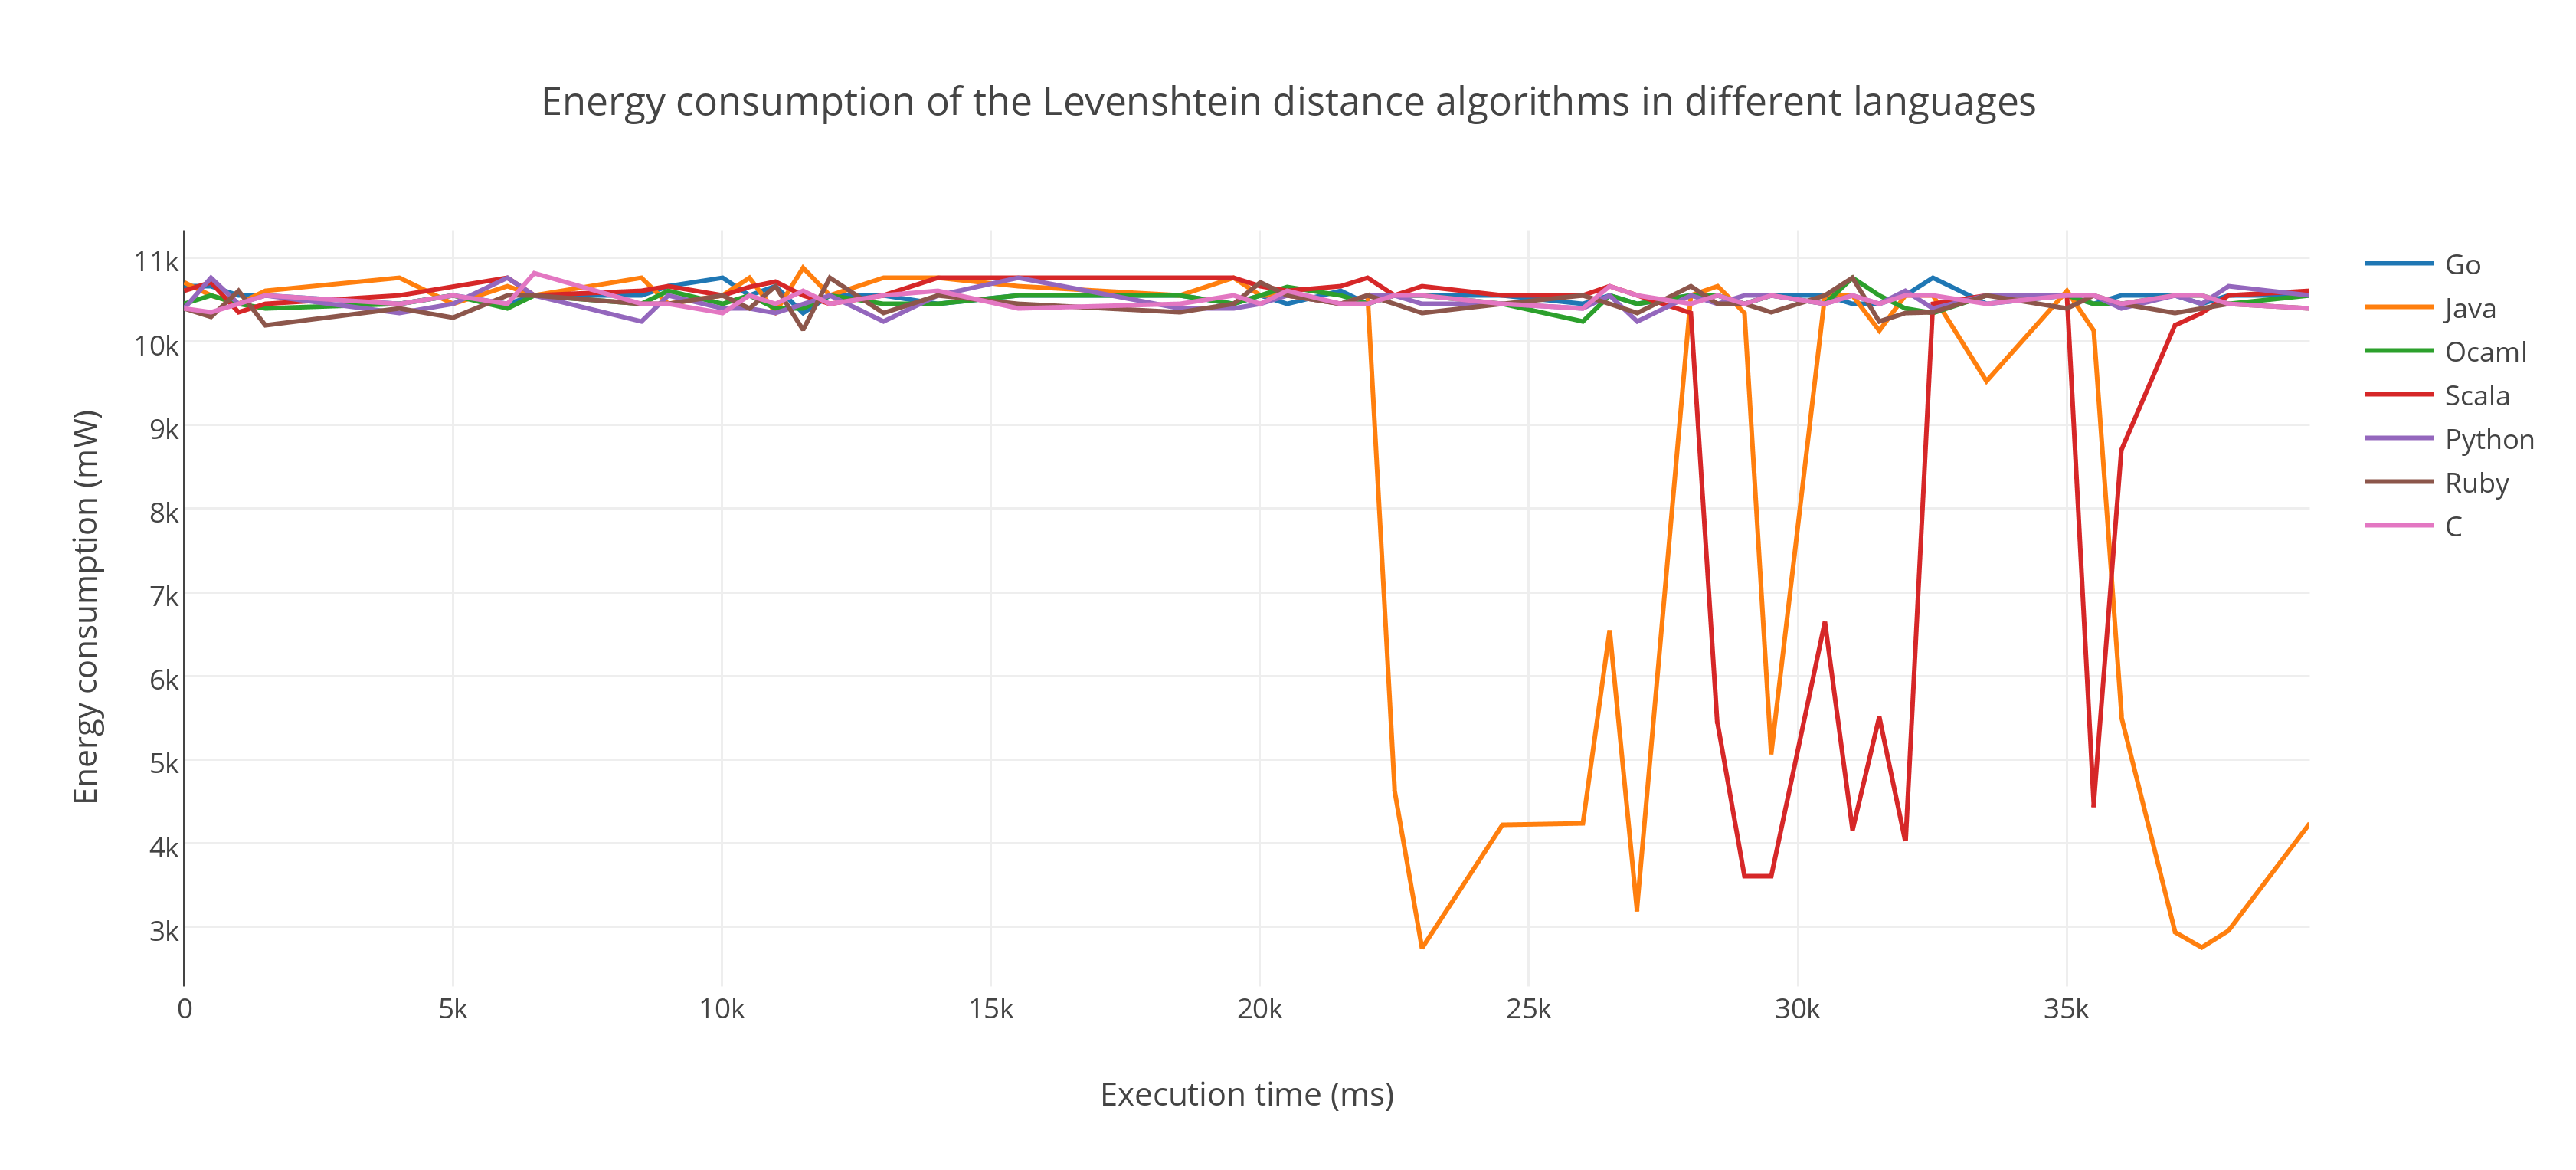
\includegraphics[width=\textwidth]{plot.png}
\end{figure}

	\subsection{Total energy consumption}
	In our context, time-dependent energy consumption is not very relevant. This aspect doesn't really reflect the efficiency of one language over another. We need to include a crucial factor, which is the execution time.
	
	If two languages have the same energy consumption, the one that takes a longer time to execute will be the least efficient. Therefore, a language is really more efficient than another if it has a smaller total energy consumption.
	
	The total energy consumption is the energy consumption in Joule, the product of the mean of energy consumptions over time with the execution time of the program. \cite{joule}
	
	\begin{figure}[H]
	\begin{gather*}
		TEC(J) = \frac{\sum\nolimits_{EC}}{\#EC} \times ET	
	\end{gather*}
	TEC = Total Energy Consumption, EC = Energy Consumption, ET = Execution Time
	\end{figure}
	
The total energy consumption of each algorithm can be found in the following figure :

\begin{figure}[H]
    \centering
    \begin{tabular}{|l|c|c|c|}
    \hline
    Language & Execution Time (s) & Mean consumption (mW) & Total consumption (J) \\
    \hline
    C & 1m32s & 10504.77 & 966\\
    Go & 1m9s & 9428.62 & 650\\
    Java & 47s & 8890.39 & 418\\
    Ocaml & 5m29s & 10358.25 & 3408\\
    Python & 7m33s & 10493.72 & 4753\\
    Ruby & 9m12s & 10468.74 & 5778\\
    Scala & 45s & 9033.88 & 406\\
    \hline
    \end{tabular}
    \caption{Total energy consumption of the algorithm in the implemented languages}
    \label{fig:tec}
    \end{figure}
    


